\documentclass[tikz,border=10pt]{standalone}
\usepackage{amsmath}
\usetikzlibrary{calc}
\begin{document}
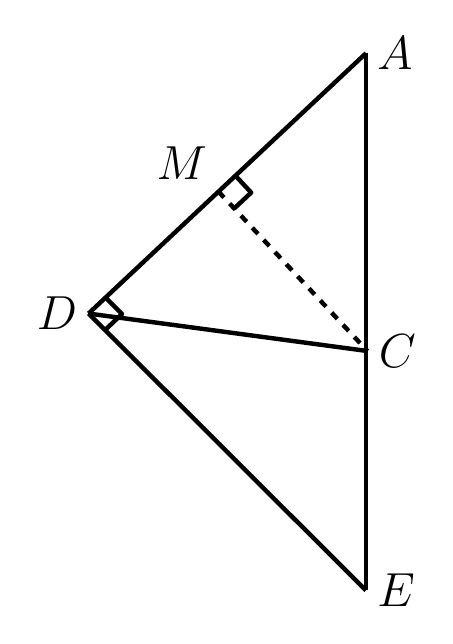
\begin{tikzpicture}[line width=1.6pt, line join=round]
  % Scale s = 0.01995 cm per px; y flipped about 446 px
  \coordinate (A) at (4.649,7.880);
  \coordinate (E) at (4.649,1.057);
  \coordinate (D) at (1.125,4.574);
  \coordinate (C) at (4.668,4.098);
  \coordinate (M) at (2.432,6.494);
  % Foot F of the perpendicular from C onto AD (start of dashed segment)
  \coordinate (F) at (2.773,6.125);

  % Right-angle mark at F (existing, verified)
  \coordinate (P1) at (2.989,6.327);
  \coordinate (P2) at (3.191,6.110);
  \coordinate (P3) at (2.975,5.908);

  % Right-angle mark at D between rays D->A and D->E (same 14.8 px square)
  \coordinate (Q1) at (1.341,4.776);
  \coordinate (Q2) at (1.550,4.568);
  \coordinate (Q3) at (1.335,4.365);

  % Solid segments
  \draw (A) -- (E);
  \draw (E) -- (D);
  \draw (A) -- (D);
  \draw (D) -- (C);

  % Dashed segment from foot F to C
  \draw[dashed] (F) -- (C);

  % Right-angle marks (one per right_angle object)
  \draw (P1) -- (P2) -- (P3);
  \draw (Q1) -- (Q2) -- (Q3);

  % Labels
  \node[right] at (A) {\fontsize{16}{19.2}\selectfont $A$};
  \node[right] at (E) {\fontsize{16}{19.2}\selectfont $E$};
  \node[left]  at (D) {\fontsize{16}{19.2}\selectfont $D$};
  \node[right] at (C) {\fontsize{16}{19.2}\selectfont $C$};
  \node[above left] at (F) {\fontsize{16}{19.2}\selectfont $M$};
\end{tikzpicture}
\end{document}